%%%%%%%%%%%%%%%%%%%%%%%%%%%%%%%%%%%%%%%%%%%%%%%%%%%%%%%%%%%%%%%%%%%%%%
% How to use writeLaTeX: 
%
% You edit the source code here on the left, and the preview on the
% right shows you the result within a few seconds.
%
% Bookmark this page and share the URL with your co-authors. They can
% edit at the same time!
%
% You can upload figures, bibliographies, custom classes and
% styles using the files menu.
%
%%%%%%%%%%%%%%%%%%%%%%%%%%%%%%%%%%%%%%%%%%%%%%%%%%%%%%%%%%%%%%%%%%%%%%

\documentclass[12pt]{article}

\usepackage{sbc-template}

\usepackage{graphicx,url}
\usepackage{xcolor}
%\usepackage[brazil]{babel}   
\usepackage[utf8]{inputenc}  

     
\sloppy

\title{Trabalho Teórico Prático\\ Teoria dos Grafos e Computabilidade}

\author{César Luiz Vales Teixeira\inst{1}, Hudsson Davih Apolinario de Andrade\inst{2}, Luís Fillipe Magalhães Conrado Pereira\inst{3} }


\address{Pontifícia Universidade Católica de Minas Gerais
  (PUCMG)\\
   -- Belo Horizonte -- MG -- Brasil
}

\begin{document} 

\maketitle

     
\begin{resumo} 
  Este artigo é a documentação do trabalho teórico prático realizado na matéria de Teoria dos Grafos e Computabilidade ministrada pelo professor Gabriel Barbosa da Fonseca. O artigo tem por objetivo explicar e documentar as decisões tomadas ao longo do trabalho.
\end{resumo}

\section{Linguagem adotada}
Todo o trabalho foi desenvolvido majoritariamente na linguagem de programação Java. Ao longo do desenvolvimento do trabalho foi necessário recorrer a elementos da linguagem Python para a geração dos gráficos quantificarmos os resultados obtidos e também para a exportação do dataset utilizado ao longo do desenvolvimento do trabalho por meio da biblioteca sklearn.

\section{Biblioteca de Grafos}

A primeira parte do trabalho consiste em uma biblioteca para manipulação de grafos. Ela possui uma classe principal, Grafo, que possui métodos para tratar arestas e vértices como definir peso e nome para cada vértice e para cada aresta, adicionar e remover arestas, testar se existe determinada aresta, se determinados vértices ou arestas são adjacentes, se o grafo é completo, se é vazio, entre outros. Ao instanciar um grafo é possível escolher a implementação, sendo as duas opções lista de adjacência e matriz de adjacência. As duas classes ListaAdjacencia e MatrizAdjacencia implementar a interface ImplementacaoGrafo, e elas representam as arestas do grafo usando uma lista e uma matriz, respectivamente. Cada uma utiliza uma classe como aresta: ArestaMatriz e ArestaLista, e as duas classes estendem a classe Aresta. Os vértices são representados por meio da classe Vertice, que assim como as classes de Aresta possuem as implementações necessárias para lidar com nome e peso de vértices ou arestas.

\section{Algoritmo de Propagação de Rótulos} 

O artigo \cite{paper}, tem por objetivo apresentar um método de aprendizado semi-supervisionado que usa uma função de classificação em relação à estrutura intrínseca revelada por pontos rotulados e não rotulados. O método apresenta um algoritmo simples para obter essa solução e mostra resultados experimentais em vários problemas de classificação. 

Com base na segunda seção do artigo, implementados o algoritmo sugerido para obter uma solução para problemas de classificação na linguagem Java como dito anteriormente. O nosso algoritmo inicia-se fazendo a leitura do dataset obtido separando as entradas e os rótulos. Após isso, replicamos o primeiro passo documentado no artigo, onde utilizamos a matriz obtida pelo dataset para calcular a distância euclidiana entre cada par de pontos de duas matrizes de números reais. Utilizaremos o resultado obtido no método RFB, cujo objetivo é calcular os pesos de uma rede neural baseada em funções de base radial (RBF), funções na qual, dependem apenas da distância entre os pontos de entrada e os centros das funções.

O segundo passo consiste em calcular a matriz de similaridade entre as linhas da matriz W, normalizando-as pelo seu comprimento. Após isso, vamos ao terceiro e último passo, cujo objetivo é calcular a iteração de uma função linear sobre a matriz de entrada, usando um fator de amortecimento alfa, no qual, foi de parametrizado em 0.99.

\section{Resultados do Algoritmo de Propagação de Rótulos}

O algoritmo foi testado com diferentes parametros para o valor alfa e de iterações. Os resultados obtidos serão mostrados a seguir:


\begin{figure}[ht]
	\centering	
	\caption[\hspace{0.1cm}Gráfico Acurácia.]{Gráfico resultado}
	\vspace{-0.4cm}
	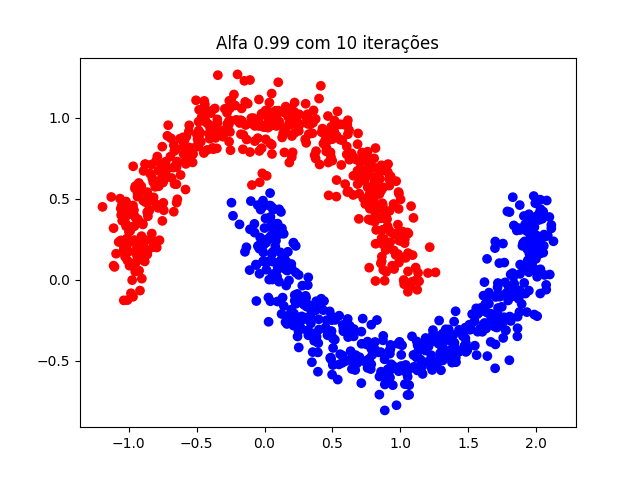
\includegraphics[width=.6\textwidth]{10_099.png}
	\\\textbf{\footnotesize  Fonte: Gráfico elaborado pelos autores }
	\label{fig:figura1}
\end{figure}

\begin{figure}[ht]
	\centering	
	\caption[\hspace{0.1cm}Gráfico Acurácia.]{Gráfico resultado}
	\vspace{-0.4cm}
	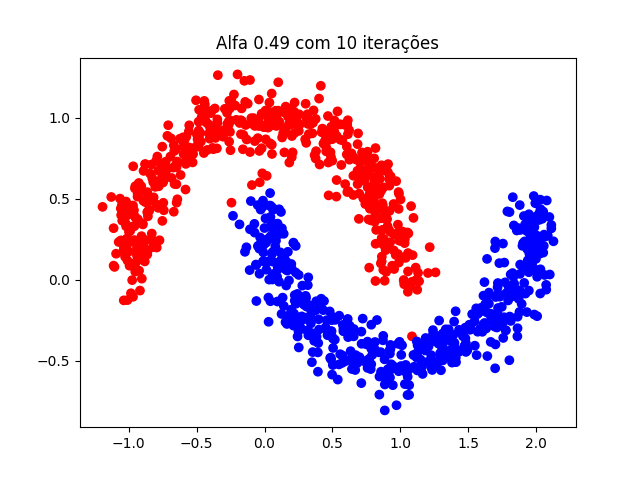
\includegraphics[width=.6\textwidth]{10_049.png}
	\\\textbf{\footnotesize  Fonte: Gráfico elaborado pelos autores }
	\label{fig:figura1}
\end{figure}

\newpage

\begin{figure}[ht]
	\centering	
	\caption[\hspace{0.1cm}Gráfico Acurácia.]{Gráfico resultado}
	\vspace{-0.4cm}
	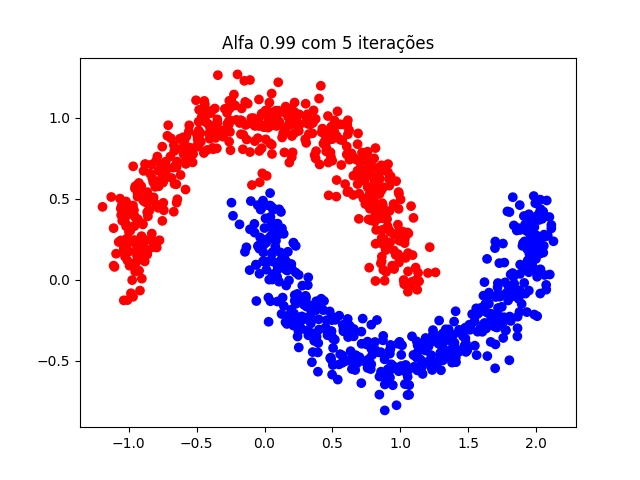
\includegraphics[width=.6\textwidth]{5_099.png}
	\\\textbf{\footnotesize  Fonte: Gráfico elaborado pelos autores }
	\label{fig:figura1}
\end{figure}

\begin{figure}[ht]
	\centering	
	\caption[\hspace{0.1cm}Gráfico Acurácia.]{Gráfico resultado}
	\vspace{-0.4cm}
	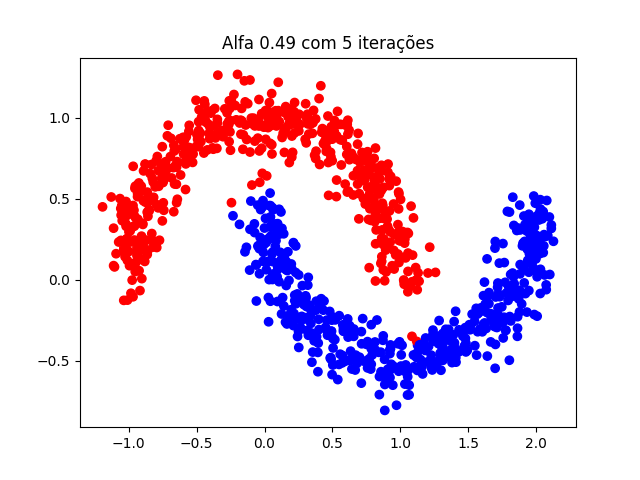
\includegraphics[width=.6\textwidth]{5_049.png}
	\\\textbf{\footnotesize  Fonte: Gráfico elaborado pelos autores }
	\label{fig:figura1}
\end{figure}

\begin{figure}[ht]
	\centering	
	\caption[\hspace{0.1cm}Gráfico Acurácia.]{Gráfico resultado}
	\vspace{-0.4cm}
	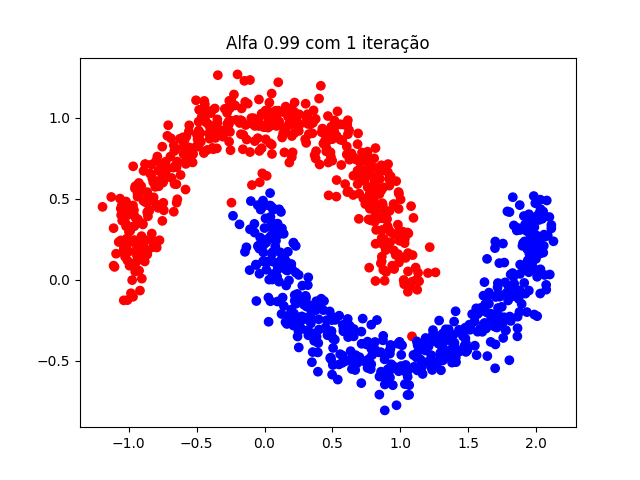
\includegraphics[width=.6\textwidth]{1_099.png}
	\\\textbf{\footnotesize  Fonte: Gráfico elaborado pelos autores }
	\label{fig:figura1}
\end{figure}

\begin{figure}[ht]
	\centering	
	\caption[\hspace{0.1cm}Gráfico Acurácia.]{Gráfico resultado}
	\vspace{-0.4cm}
	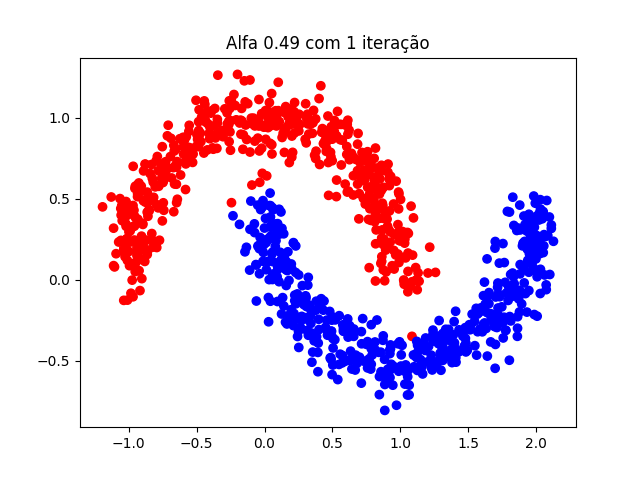
\includegraphics[width=.6\textwidth]{1_049.png}
	\\\textbf{\footnotesize  Fonte: Gráfico elaborado pelos autores }
	\label{fig:figura1}
\end{figure}
\newpage

\begin{itemize}
\color{white}
\item First item
\item Second item
\end{itemize}
\newpage
Em resumo esse foi os dados obtidos durante a execução do nosso algoritmo:
\begin{table}[ht]
\centering
\caption{Dados obtidos durante os testes}
\label{tab:exTable1}
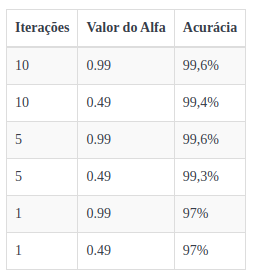
\includegraphics[width=.45\textwidth]{tabela.png}
\\\textbf{\footnotesize  Fonte: Tabela elaborada pelos autores }
\end{table}

Podemos observar que, mesmo com a variação de iterações e do valor de alfa, o nosso algoritmo se manteve com uma acurácia alta, tendo seu menor resultado encontrado quando simulado com apenas 1 iteração e com um alfa de 0.49.

\section{Divisão das tarefas no trabalho}
Ao longo do trabalho todos os integrantes do grupo realizaram todas as tarefas em conjunto. Mas em especial César atuou na implementação do algoritmo de propagação de rótulos, Hudsson atuou na biblioteca de grafos e na elaboração deste artigo e Luís Fillipe atuou junto ao César na implementação do algoritmo de propagação e junto ao Hudsson na elaboração deste artigo
\newpage\newpage
\bibliographystyle{sbc}
\bibliography{sbc-template}

\end{document}
